
\chapter[ಭಾಗ -  2]{}\label{chap2}

\begin{center}
\rule{5cm}{1pt}\\[5pt]
{\Large\bfseries ಅಲಂಕಾರಿಕ ವಸ್ತುಗಳ ತಯಾರಿಕೆ }\\[3pt]
\rule{5cm}{1pt}
\end{center}
 
 \begin{itemize}
 \item ನಿರ್ದಿಷ್ಟ ಮಾನ ಆಕಾರಗಳು (6 ರೀತಿಯಲ್ಲಿ)
 \item  ಮೀನನ ರಚನೆ
 \item Flower for Rose
 \item Six point star
 \item ಮಾಘ ಮಾಲೆ
 \item ಹಡಗ ತಯಾರಿಕೆ
 \item ದ್ವಿಪಾದ ಹಡಗು
 \item wind mill
 \item ಟ್ರೇ
 \item ಕಪ್ 
 \item samurais Helmet
 \item  yakka-San.
  \end{itemize}
 
 \section*{ಓರಿಗಾಮಿಯಲ್ಲಿ ನಿರ್ದಿಷ್ಟ ಮಾನ ಆಕಾರಗಳು [Standard Shapes]}
 
 ಈಗ ಸಾವಿರಾರು ಕಾಗದದ ಮಾದರಿಗಳನ್ನು ತಯಾರಿಸುವುದನ್ನು ತಿಳಿದುಕೊಂಡಿದ್ದೇವೆ. ಈ ಕಾಗದ ಮಾದರಿಗಳನ್ನು ತಯಾರಿಸುವಾಗ ಅನೇಕ ಹಂತಗಳಲ್ಲಿ ಕಾಗದವನ್ನು ಮಡಚಬೇಕಾಗುತ್ತದೆ. ಹೀಗೆ ಮಡಚಬೇಕಾದರೆ, ಒಂದು ನಿರ್ದಿಷ್ಟ ಆಕಾರದ ಮಡಚುವಿಕೆಯನ್ನು ಪ್ರಾರಂಭದ ಹಂತದಲ್ಲಿ ಬಳಸುತೇವೆ. ಈ ರೀತಿಯ ಮಡಚುವಿಕೆಯನ್ನು "ನಿರ್ದಿಷ್ಟ ಮಾನ ಆಕಾರಗಳು" [Standard shapes] ಎಂದು ಕರೆಯುತ್ತೇವೆ. ಮುಖ್ಯವಾಗಿ `S' ನಿರ್ದಿಷ್ಟ ಮಾನ ಆಕಾರಗಳು ಇರುತ್ತವೆ. ಅವು ಒಂದಕ್ಕೊಂದು ಆಂತರಿಕವಾಗಿ ಸಂಬಂಧ ಹೊಂದಿರುತ್ತವೆ. ಅವು ಕೆಳಗಿನಂತೆ ಇರುತ್ತವೆ. 
  \begin{enumerate}
  \item[{\bf [1]}] \textbf{Waterbomb Base :} ಇದೊಂದು ಪ್ರಾರಂಭದ ನಿರ್ದಿಷ್ಟಮಾನ ಆಕಾರವಾಗಿದೆ. ಇದರ 5 ಬಿಂದುಗಳು ಅನೇಕ ನಕ್ಷೆಗಳಿಗೆ ಪರಿವರ್ತನ ಶೀಲ ಆಕಾರಗಳನ್ನು ಮಾಡುತ್ತವೆ. ಇದರಿಂದ "water bomb"ನ್ನು ತಯಾರಿಸಬಹುದು.
  
  \item[{\bf [2]}] \textbf{Preliminary Base:} ಇದು ಅನೇಕ ನಿರ್ದಿಷ್ಟ ಮಾನ ಆಕಾರಗಳಿಗೆ ಪ್ರಾರಂಭದ ಹಂತವಾಗಿರುತ್ತದೆ. ಅಂದರೆ ಇದರಿಂದ "Bird Base" "Frog/lily Base" "paper crane", "Tato, Flopping Bird"  ಮುಂತಾದವುಗಳನ್ನು ತಯಾರಿಸಬಹುದು.  
  
  \item[{\bf [3]}] \textbf{Frog/lily Base:} ಇದು ದಿಂದ ಪ್ರಾರಂಭವಾಗುತ್ತದೆ. ಅಂದರೆ ಈ ವಿಧಾನದಿಂದ ಮತ್ತು ಗಳನ್ನು ತಯಾರಿಸಬಹುದು.
   
  \item[{\bf [4]}] \textbf{Bird  Base:} ಇದು ಯ ಪ್ರಾರಂಭದ ಹಂತವಾಗಿದೆ. ಇದರಿಂದ ಅನೇಕ ಪಕ್ಷಿಗಳನ್ನು/ಪ್ರಾಣಿಗಳನ್ನು ತಯಾರಿಸಬಹುದು. 
  
  \item[{\bf [5]}] \textbf{Fish Base:}  ಇದು ಅನೇಕ ಸಂಕೀರ್ಣ ಮಾದರಿಗಳ ತಯಾರಿಕೆಯಲ್ಲಿ ಪ್ರಾರಂಭದ ಹಂತವಾಗಿರುತ್ತದೆ. ಇದರಿಂದ "ಪಾರಂಪರಿಕ ಮೀನ್"ದ ಮಾದರಿಯನ್ನು ರಚಿಸಬಹುದು.
  
  \item[{\bf [6]}] \textbf{ಗಾಳಿಪಟ ಅಡಿಪಾಯ : Kite Base:} ಇದೊಂದು ಮುಖ್ಯವಾದ ಅಡಿಪಾಯವಾಗಿದೆ. ಇದರಿಂದ ವಿವಿಧ ರೀತಿಗಳಲ್ಲಿ ಕಾಗದವನ್ನು ಮಡಚಿ ವಿವಿಧ ರೀತಿಯ ಪಕ್ಷಿಗಳನ್ನು ತಯಾರಿಸಲು ಬರುತ್ತದೆ. 
     \end{enumerate}
\begin{enumerate}
\item[{\bf [1]}] \textbf{ವಾಟರ್ ಬಾಂಬು ಅಡಿಪಾಯ  [Water bomb Base]}
\begin{figure}[H]
\centering
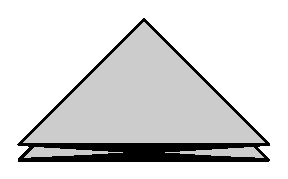
\includegraphics[scale=.98]{src/figure/chap2/fig2-1a.eps}
\end{figure}
\begin{figure}[H]
\centering
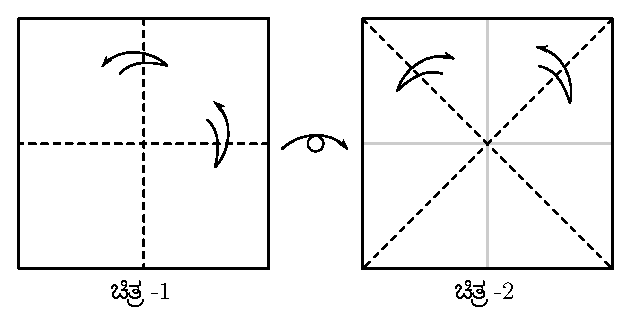
\includegraphics[scale=.98]{src/figure/chap2/fig2-1b.eps}\\
\textbf{1. ಬಣ್ಣದ ಬದಿ ಮೇಲೆ ಇರುವಂತೆ ಚಿತ್ರದಲ್ಲಿ ತೋರಿಸಿದಂತೆ ಮಡಚಿ ತೆಗೆಯಬೇಕು.}\\
\textbf{2. ಕರ್ಣದ ಗುಂಟ ಮಡಚಿ ಬಿಚ್ಚಬೇಕು.}
\end{figure}
\begin{figure}[H]
\centering
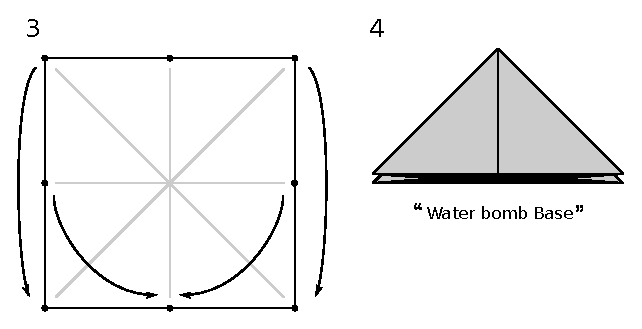
\includegraphics[scale=.98]{src/figure/chap2/fig2-1c.eps}
\end{figure}


\item[{\bf [2]}] \textbf{Preliminary Base: "ಪ್ರಾರಂಭಿಕ ಅಡಿಪಾಯ"}
ಈ ವಿಧಾನವನ್ನು ಪಕ್ಷಿಗಳ, ಕಪ್ಪೆ  ಮತ್ತು `ಲಿಲ್ಲಿ' ಹೂಗಳನ್ನು ತಯಾರಿಸಲು ಅಡಿಪಾಯವಾಗಿದೆ. ಇದು ಹೆಚ್ಚು ಸಾಮಾನ್ಯ ವಿಧಾನವಾಗಿದೆ. 
\begin{figure}[H]
\centering
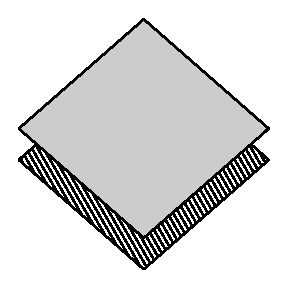
\includegraphics[scale=.98]{src/figure/chap2/fig2-2.eps}
\end{figure}

\textbf{ಮಡಚುವ ಹಂತಗಳು :}
\begin{figure}[H]
\centering
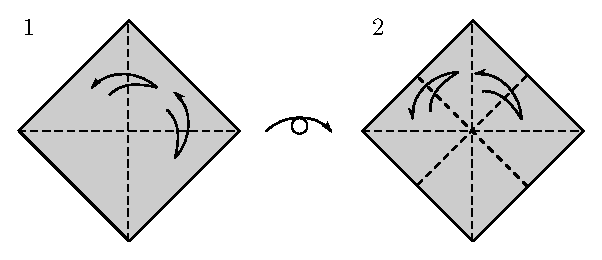
\includegraphics[scale=.98]{src/figure/chap2/fig2-2a.eps}
\end{figure}
\begin{figure}[H]
\centering
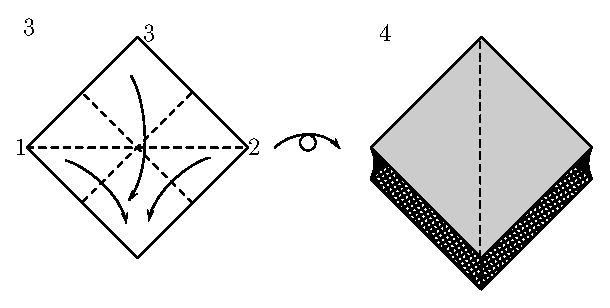
\includegraphics[scale=.98]{src/figure/chap2/fig2-2b.eps}
\end{figure}

\item[{\bf [3]}] \textbf{Frog/Lily Base :} ಇದು "Preliminary base" ವಿಧಾನದಿಂದ ಪ್ರಾರಂಭವಾಗುತ್ತದೆ.
\begin{figure}[H]
\centering
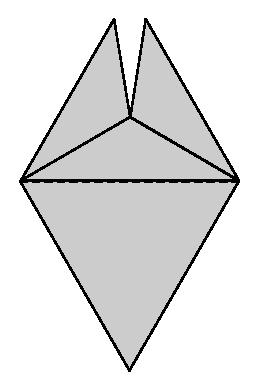
\includegraphics[scale=.98]{src/figure/chap2/fig2-3.eps}
\end{figure}

ಅಂದರೆ, "Preliminary Base" ವಿಧಾನವು ಪೂರ್ಣಗೊಂಡ ನಂತರ ಈ ಮಡಚುವ ಹಂತಗಳು ಪ್ರಾರಂಭವಾಗುತ್ತವೆ.

ಇಲ್ಲಿ ಒಂದು ಬದಿಬಣ್ಣದ ಹಾಗೂ ಇನ್ನೊಂದು ಬದಿ ಬಿಳಿ ಬಣ್ಣವಿರುವ ಕಾಗದವನ್ನು ಚೌರಸ ಆಕಾರದಲ್ಲಿ ತೆಗೆದುಕೊಂಡು ಪ್ರಾರಂಭ ಮಾಡಬೇಕು.

\textbf{ಮಡಚುವ ಹಂತಗಳು :}
\begin{figure}[H]
\centering
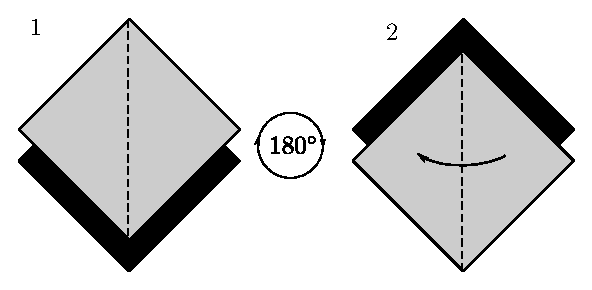
\includegraphics[scale=.98]{src/figure/chap2/fig2-3a.eps}\\
\textbf{1. Preliminary Base ಮುಗಿದಾಗ ಬಣ್ಣದ ಭಾಗವು ಮೇಲೆ ಬರುತ್ತದೆ.}\\
\textbf{2. ಹಂತ 1ನ್ನು $180^{\circ}$ ಕೋನ ಮಾಡಿ ತಿರುಗಿಸಬೇಕು. ತೆರೆದ ಭಾಗ ಮೇಲೆ ಬರುತ್ತದೆ.}
\end{figure}
\begin{figure}[H]
\centering
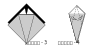
\includegraphics[scale=.98]{src/figure/chap2/fig2-3b.eps}\\
\textbf{3. ಒಂದು ಬದಿಯಲ್ಲಿ ಚಿತ್ರದಲ್ಲಿ ತೋರಿಸಿದಂತೆ ಮಡಚಬೇಕು. ಉಳಿದ ಭಾಗಗಳನ್ನು ಮಡಚಬೇಕು.}\\
\textbf{4. ಮೇಲಿನ ಪದರನ್ನು ಮಾತ್ರ ಮಧ್ಯದ ಗೆರೆಯಗೆ ಮಡಚಬೇಕು.}
\end{figure}
\begin{figure}[H]
\centering
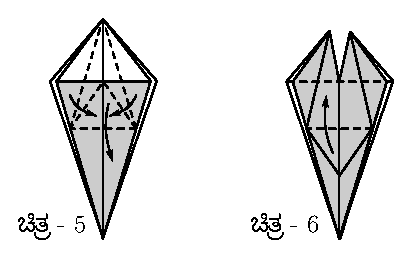
\includegraphics[scale=.98]{src/figure/chap2/fig2-3c.eps}\\
\textbf{5. ದಳದ ಮಡಿಕೆ. ಮೇಲಿನ ಪದರನ್ನು ಪೂರ್ಣವಾಗಿ ಕೆಳಮುಖ ಮಡಚಬೇಕು ಮತ್ತು ಮಧ್ಯದ ಗೆರೆಗೆ ಬದಿಗಳನ್ನು ಮಡಚಬೇಕು. ಕೊನೆಗೆ ಉಬ್ಬು ಮಡಿಕೆ ಮಾಡಬೇಕು.}\\
\textbf{6. ದಳದ ಮಡಿಕೆಯನ್ನು ಮುಗಿಸಿ, ತಗ್ಗು ಮಡಿಕೆ ಮಾಡಿ ತ್ರಿಭುಜ ಆಕಾರದ ಭಾಗವನ್ನು ಮೇಲಕ್ಕೇ ಮಡಚಬೇಕು. ಮತ್ತು 4 ಮತ್ತು 6 ಹಂತಗಳನ್ನು ಉಳೀದ 3ಬದಿಗಳಲ್ಲಿ ಮಾಡಿ ಮುಗಿಸಬೇಕು.}
\end{figure}
\begin{figure}[H]
\centering
\includegraphics[scale=.98]{src/figure/chap2/fig2-3d.eps}\\
\textbf{7. ಈಗ Frog/Lily ಮಡಿಕೆ. ಪೂರ್ಣವಾಗಿದೆ.}
\end{figure}

\item[{\bf [4]}] \textbf{ಪಕ್ಷಿ ಮಾದರಿ [Bird Base] ಮಡುಚುವಿಕೆ: ಪಕ್ಷಿ ಅಡಿಪಾಯ}
\begin{figure}[H]
\centering
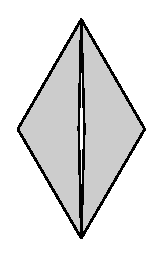
\includegraphics[scale=.98]{src/figure/chap2/fig2-4.eps}\\
\end{figure}

ವಿವಿಧ ರೀತಿಯ ಪಕ್ಷಿಗಳನ್ನು ಹಾಗೂ ಪ್ರಾಣಿಗಳ ಮಾದರಿಗಳನ್ನು ತಯಾರಿಸಲು ಈ ಪಕ್ಷಿ ಮಾದರಿ ಮಡಿಕೆ ಉಪಯೋಗವಾಗುತ್ತದೆ. ಇದು "preliminary Base"ದಿಂದ ಮುಂದುವರಿಯುತ್ತವೆ. 

\begin{figure}[H]
\centering
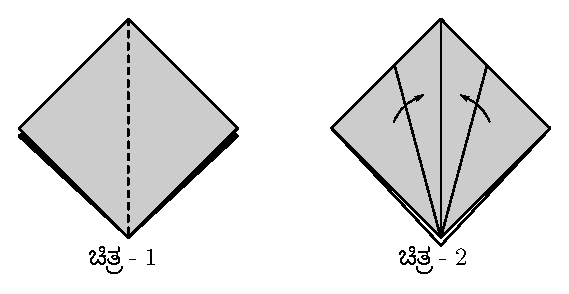
\includegraphics[scale=.98]{src/figure/chap2/fig2-4a.eps}\\
\textbf{1. "Preliminary Base"ದಿಂದ ಮಡಿಕೆಯನ್ನು ಮುಂದುವರಿಸಬೇಕು.}\\
\textbf{2. ಮೇಲಿನ ಪದರನ್ನು ಮಧ್ಯದ ಗೆರೆಗೆ ಮಡಚಬೇಕು.}
\end{figure}
\begin{figure}[H]
\centering
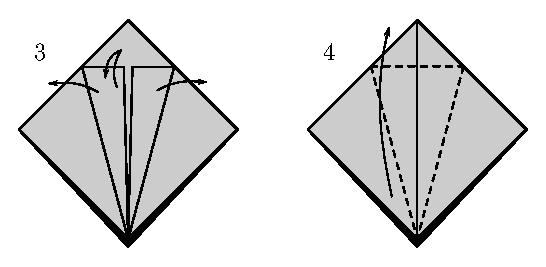
\includegraphics[scale=.98]{src/figure/chap2/fig2-4b.eps}\\
\textbf{3. ಮೇಲಿನ ತ್ರಿಭುಜವನ್ನು ಮಡಚಿರಿ.}\\
\textbf{4. ಮೇಲಿನ ಪದರನ್ನು ಮೇಲಕ್ಕೆ ಎತ್ತಿರಿ.}
\end{figure}
\begin{figure}[H]
\centering
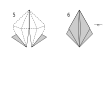
\includegraphics[scale=.98]{src/figure/chap2/fig2-4c.eps}\\
\textbf{5. 4ನೇ ಹಂತವು ಮುಂದುವರಿದಿದೆ. ಮಾದರಿಯು '3' ಆಯಾಮ ಆಗಿರುತ್ತದೆ. ಇರು:ದು ಗೆರೆಗಳ ಮೂಲಕ ಮೇಲಿನ ಪದರಗಳನ್ನು ಒಳಭಾಗದಲ್ಲಿ ಮಡಚಿರಿ.}\\
\textbf{6. 4ನೇ ಹಂತವು ಪೂರ್ಣವಾಗಿದ್ದು ಮಾದರಿಯು ಸಮತಟ್ಟಾವಾಗಿರುತ್ತದೆ. ಮಾದರಿಯನ್ನು ತಿರುವು ಮುರುವು ಮಾಡಿರಿ.}
\end{figure}
\begin{figure}[H]
\centering
\includegraphics[scale=.98]{src/figure/chap2/fig2-4d.eps}\\
\textbf{7. ಮತ್ತೊಂದು ಬದಿಯಲ್ಲಿ 2ರಿಂದ 6ರ ವರಗಿನ ಹಂತಗಳನ್ನು ಪೂನಾವರ್ತನೆ ಮಾಡಬೇಕು.}\\
\textbf{8. ಪಕ್ಷಿ ಮಡಿಕೆ. (Bird Base) ಮುಗಿದಾಗ ಮಾದರಿ.}
\end{figure}

\item[{\bf [5]}] {\textbf Fish Base : "ಮೀನು ಅಡಿಪಾಯ"}

ಒಂದು ಬದಿಬಣ್ಣದ ಇನ್ನೊಂದು ಬದಿ ಬಳಿ ಇರುವ ಚೌರಸ ಆಕಾರದ ಕಾಗದ ತೆಗೆದುಕೊಂಡು ಕೆಳಗಿನಂತೆ ಮಡಚಬೇಕು.

\begin{figure}[H]
\centering

\includegraphics[scale=.98]{src/figure/chap2/fig2-5a.eps}\\
\textbf{1. ಬಿಳಿಭಾಗ ಮೇಲೆ ಬರುವಂತೆ ಹಿಡಿದು ಒಂದು ಕರ್ಣದಗುಂಟ ಮಡಚಿ ತೆರೆಯಬೇಕು.}\\
\textbf{2. ನಂತರ ಕರ್ಣದ ಒಂದು ಬಿಂದುವಿನಿಂದ ಎರಡು ಶೃಂಗಬಿಂದುಗಳನ್ನು ಮಧ್ಯ ರೇಖೆಗೆ ಹೊಂದುವಂತೆ ಮಡಬೇಕು.}
\end{figure}
\begin{figure}[H]
\centering
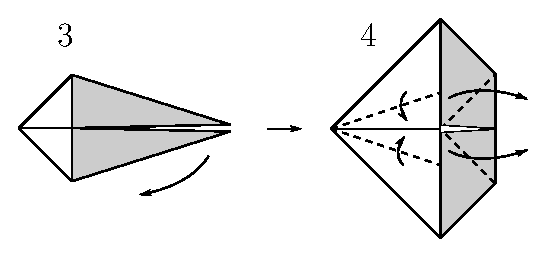
\includegraphics[scale=.98]{src/figure/chap2/fig2-5b.eps}\\
\textbf{3. ಹಿಂಬದಿಗೆ ಅರ್ಧಭಾಗ ಉಬ್ಬು ಮಡಿಕೆ ಮಾಡಬೇಕು.}\\
\textbf{4. ಎರಡು ಬದಿಯಲ್ಲಿ 'Squash Fold' ಮಾಡಬೇಕು.}
\end{figure}
\begin{center}[H]
%\includegraphics[scale=.98]{src/figure/chap2/fig2-5c.eps}\\
\textbf{5. ಹಿಂದಿನ ಪದರನ್ನು ಹಿಂಬದಿಗೆ ಉಬ್ಬು ಮಡಿಕೆ ಮಾಡಬೇಕು. }\\
\textbf{6. 'Fish Base' ಮಾದರಿ}
\end{center}

\item[{\bf [6]}] {\textbf ಗಾಳಿಪಟ ಅಡಿಪಾಯ : [Kite Base]}

ಒಂದು ಬದಿ ದಟ್ಟಬಣ್ಣ ಇನ್ನೊಂದು ಬದಿ ಬಿಳಿ ಅಥವಾ ತೆಳುಬಣ್ಣದ ಚೌಕಾಕಾರದ ಹಾಳೆಯಿಂದ ಕೆಳಗಿನಂತೆ ಮಡಚಿ ಗಾಳಿಪಟ ಅಡಿಪಾಯವನ್ನು ಮಾಡಬಹುದು. 

\textbf{ಮಡಚುವ ಹಂತಗಳು :}
\begin{figure}[H]
\centering
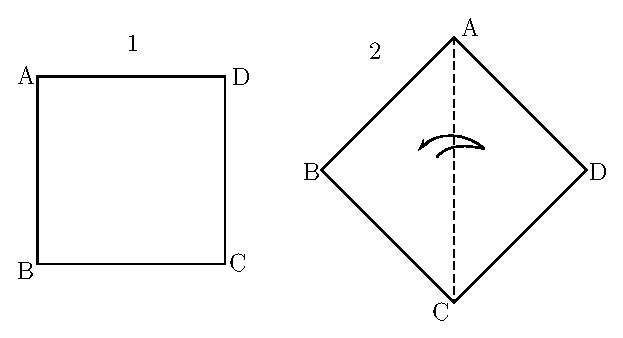
\includegraphics[scale=.98]{src/figure/chap2/fig2-6a.eps}\\
\textbf{1. ಬಿಳಿ ಅಥವಾ ತೆಳುಬಣ್ನದ ಬದಿ (ಮೈ) ಮೇಲೆ ಬರುವಂತೆ ಹಿಡಿಯಬೇಕು.}\\
\textbf{2. AC ಕರ್ಣದ ಗುಂಟ ಮಡಚಿ ನಂತರ ಬಿಚ್ಚಬೇಕು.}
\end{figure}
\begin{figure}[H]
\centering
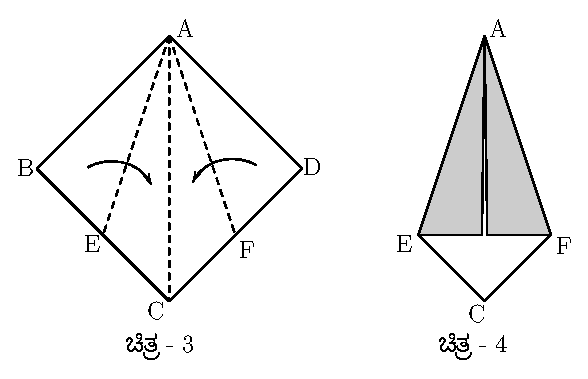
\includegraphics[scale=.98]{src/figure/chap2/fig2-6b.eps}\\
\textbf{3. AB ಮತ್ತು AD ಬಾಹುಗಳನ್ನು  AC ಕರ್ಣಕ್ಕೆ ಸರಿಯಾಗಿ ಹೊಂದುವಂತೆ ಮಡಚಬೇಕು.}\\
\textbf{4. ಗಾಳಿಪಟ ಅಡಿಪಾಯ [Kite Base] ತಯಾರಾಯಿತು. ಈ 4 ಹಂತಗಳಿಂದ ಮುಂದುವರಿಸಿ ಅನೇಕ ಪಕ್ಷಿಗಳನ್ನು ತಯಾರಿಸಬಹುದು.}
\end{figure}

\section*{ಅಲಂಕಾರಿಕ ವಸ್ತುಗಳ ಮಾದರಿಗಳ ತಯಾರಿಕೆ}

ಗಾಳಿಪಟ ಅಡಿಪಾಯವನ್ನು ಮುಂದುವರಿಸಿ ಈ ಮಾದರಿಯನ್ನು ಕೆಳಗಿನಂತೆ ತಯಾರಿಸಬಹುದು.
\begin{figure}[H]
\centering
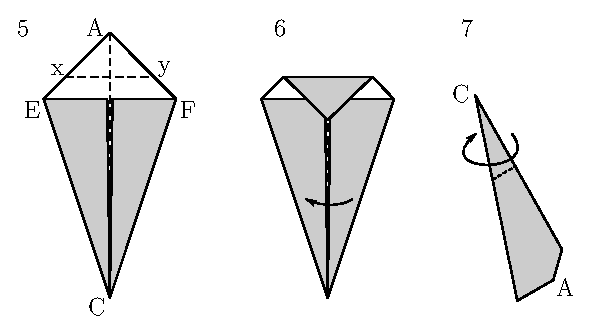
\includegraphics[scale=.98]{src/figure/chap2/fig2-6c.eps}\\
\textbf{5. xy ಗೆರೆಯ ಗುಂಟ A ಬಿಂದುವನ್ನು ಮುಂದೆ ಮಡಿಚಬೇಕು.}\\
\textbf{6. AC ಕರ್ಣದ ಗುಂಟ ಒಳಮುಖವಾಗಿ ಮಡಚಬೇಕು.}\\
\textbf{7. C ಬಿಂದು ACಗೆ ಲಂಬವಾಗಿರುವಂತೆ ಮಡಚಬೇಕು.}
\end{figure}
\begin{figure}[H]
\centering
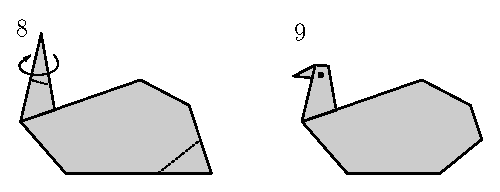
\includegraphics[scale=.98]{src/figure/chap2/fig2-6d.eps}\\
\textbf{8. ಎರಡು ಜಾಗೆಗಳಲ್ಲಿ ಗೆರೆಗಳ ಗುಂಟ ಮಡಚಬೇಕು.}
\end{figure}

"ಗಾಳಿಪಟ ಅಡಿಪಾಯ"ವನ್ನು ಮುಂದುವರಿಸಿ ಈ ಮಾದರಿಯನ್ನು ಕೆಳಗಿನಂತೆ ತಯಾರಿಸಬೇಕು.
\begin{figure}[H]
\centering
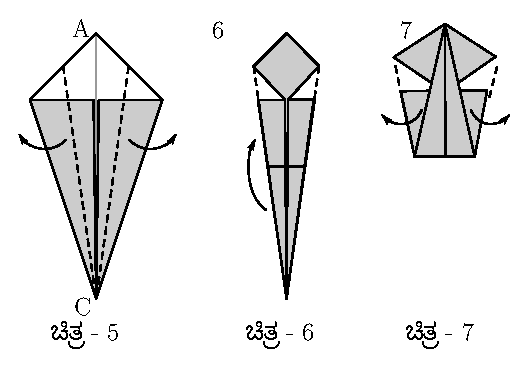
\includegraphics[scale=.98]{src/figure/chap2/fig2-6e.eps}
\end{figure}
\begin{figure}[H]
\centering
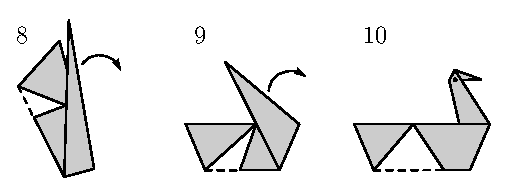
\includegraphics[scale=.98]{src/figure/chap2/fig2-6f.eps}
\end{figure}

ಗಾಳಿಪಟ ಅಡಿಪಾಯ [Kite base] ಉಪಯೋಗಿಸಿ ಈ ಮಾದರಿಯನ್ನು ಕೆಳಗಿನಂತೆ ತಯಾರಿಸಬಹುದು.
\begin{figure}[H]
\centering
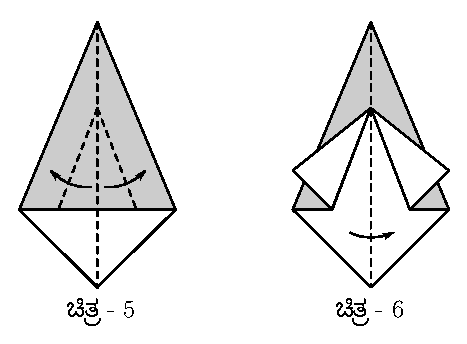
\includegraphics[scale=.98]{src/figure/chap2/fig2-6g.eps}
\end{figure}
\begin{figure}[H]
\centering
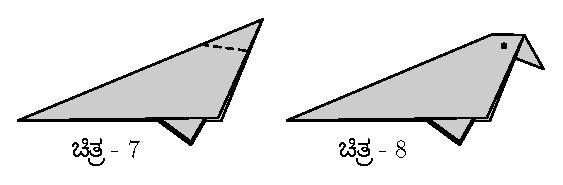
\includegraphics[scale=.98]{src/figure/chap2/fig2-6h.eps}
\end{figure}

ಗಾಳಿಪಟ ಅಡಿಪಾಯ [Kite base]ದ ಸಹಾಯದಿಂದ ಕೆಳಗಿನಂತೆ ಮಡಚಿ ಪಕ್ಷಿಯ ಮಾದರಿಯನ್ನು ತಯಾರಿಸುವುದು. 
\begin{figure}[H]
\centering
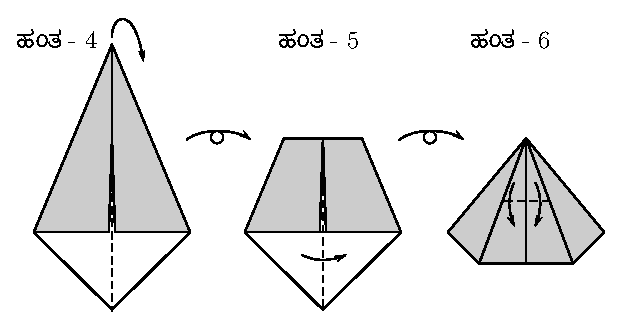
\includegraphics[scale=.98]{src/figure/chap2/fig2-6i.eps}
\end{figure}
\begin{figure}[H]
\centering
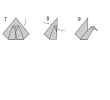
\includegraphics[scale=.98]{src/figure/chap2/fig2-6j.eps}
\end{figure}
\end{enumerate}

\medskip
\noindent
\textbf{ಮೀನು [Fish]}
\begin{figure}[H]
\centering
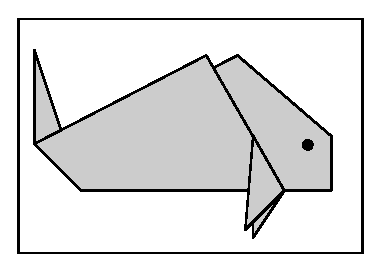
\includegraphics[scale=.98]{src/figure/chap2/fig2-7.eps}
\end{figure}

\textbf{ಮಡಚುವ ಹಂತಗಳು :}
\begin{figure}[H]
\centering
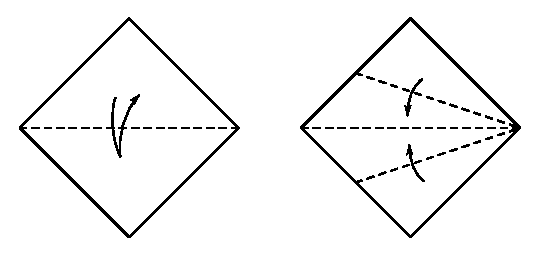
\includegraphics[scale=.98]{src/figure/chap2/fig2-7a.eps}\\
\textbf{1. ಬಿಳಿಭಾಗವು ಮೇಲೆ ಬರುವಂತೆ ಹಿಡಿದು ಕರ್ಣದ ಗುಂಟ ಮಡಚಿ ಬಿಚ್ಚಬೇಕು.}\\
\textbf{2. ಅಡ್ಡ ಗೆರೆಯ ಮೇಲಿನ ಮತ್ತು ಕೆಳಗಿನ ಶೃಂಗಗಳನ್ನು ಮಧ್ಯ ಗೆರೆಗೆ ಹೊಂದುವಂತೆ ಮಡಚಬೇಕು.}
\end{figure}
\begin{figure}[H]
\centering
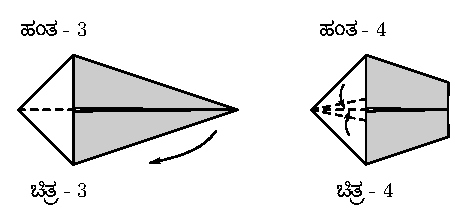
\includegraphics[scale=.98]{src/figure/chap2/fig2-7b.eps}\\
\textbf{3. ಬಲಭಾಗದ ಶೃಂಗವನ್ನು ಹಿಂದಕ್ಕೆ ಅರ್ಧಭಾಗಕ್ಕೆ ಸರಿಯಾಗುವಂತೆ ಮಡಚಬೇಕು.}\\
\textbf{4. ಚಿತ್ರದಲ್ಲಿ ತೋರಿಸಿದಂತೆ ಎರಡು ಬದಿಯನ್ನು ಮಧ್ಯ ರೇಖೆಗೆ ಹೊಂದುವಂತೆ ಮಡಚಿ. ಹಿಂದೆ ಹಾಗೂ ಮುಂದಿನ ಭಾಗಗಳನ್ನು ಮೊದಲಿನಂತೆ ಮಾಡಬೇಕು.}
\end{figure}
\begin{figure}[H]
\centering
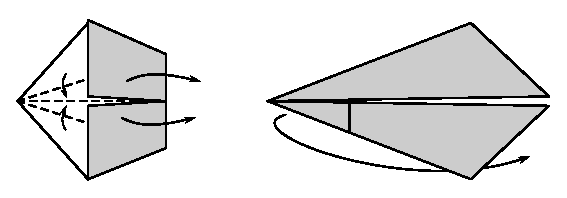
\includegraphics[scale=.98]{src/figure/chap2/fig2-7c.eps}\\
\textbf{6. ಹಿಂದಿನ ಪದರನ್ನು ಹಿಂದಕ್ಕೆ ಉಬ್ಬು ಮಡಿಕೆ ಮಾಡಬೇಕು.}
\end{figure}
\begin{figure}[H]
\centering
\includegraphics[scale=.98]{src/figure/chap2/fig2-7d.eps}\\
\textbf{7. ಉಬ್ಬು ಮಡಿಕೆಯನ್ನು (ಗೆರೆಯ ಗುಂಟ) ಹಿಂಬದಿಗೆ ಮಾಡಬೇಕು. ಇದು "Fish base" ಆಗಿದೆ.}\\
\textbf{8. ಅರ್ಧಕ್ಕೆ ಉಬ್ಬು ಮಡಿಕೆ ಮಾಡಬೇಕು.}
\end{figure}
\begin{figure}[H]
\centering
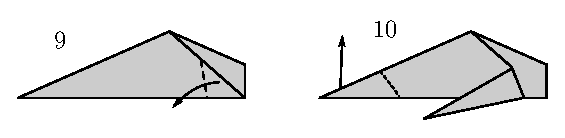
\includegraphics[scale=.98]{src/figure/chap2/fig2-7e.eps}\\
\textbf{9. ಹಕ್ಕಿಗಳನ್ನು ಕೆಳಕ್ಕೆ ಮಡಚಬೇಕು.}\\
\textbf{10. ಗೆರೆಯಗುಂಟ ಹಿಂಬದಿಗೆ ಮಡಚಬೇಕು.}
\end{figure}
\begin{figure}[H]
\centering
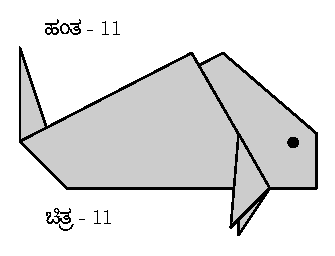
\includegraphics[scale=.98]{src/figure/chap2/fig2-7f.eps}\\
\textbf{11. "ಮೀನ್‌ನ ಮಾದರಿ" Fish Model}
\end{figure}

\medskip
\noindent
\textbf{Flower for Rose}
\begin{figure}[H]
\centering
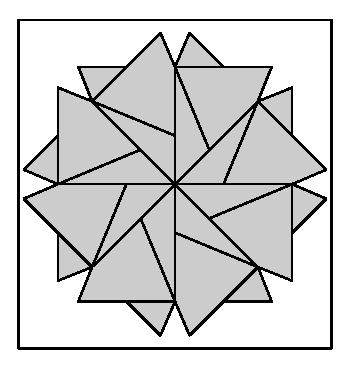
\includegraphics[scale=.98]{src/figure/chap2/fig2-8.eps}
\end{figure}

\textbf{ಮಡಚುವ ಹಂತಗಳು :}
\begin{figure}[H]
\centering
\includegraphics[scale=.98]{src/figure/chap2/fig2-8a.eps}\\
\textbf{1. ಚೌರಸದ ಬಿಳಿಭಾಗವು ಮೇಲೆ ಇರುವಂತೆ ಒಂದು ಕರ್ಣದ ಗುಂಟ ಮಡಚಿ ಬಿಚ್ಚಬೇಕು.}\\
\textbf{2. ಹಂತ 1ರಲ್ಲಿ ಮಾಡಿದ ಗೆರೆಯ ಗುಂಟ ಎರಡು ಬದಿಗಳನ್ನು ಮಡಚಿ ಬಿಚ್ಚಬೇಕು.}
\end{figure}
\begin{figure}[H]
\centering
\includegraphics[scale=.98]{src/figure/chap2/fig2-8b.eps}\\
\textbf{3. ಹಂತ 2ರಲ್ಲಿ ಮಾಡಿದ ಗೆರೆಗಳಿಗೆ ಹೊಂದಿಕೊಂಡು ಮೇಲಿನ ತುದಿಯನ್ನು ಕೆಳಮುಖವಾಗಿ ಮಡಚಬೇಕು.}\\
\textbf{4. ಹಂತ 3ರಲ್ಲಿ ಮಾಡಿದ ಗೆರೆಯ ಗುಳ ಎರಡು ಬದಿಗಳಲ್ಲಿ ಮಡಚಬೇಕು.}
\end{figure}
\begin{figure}[H]
\centering
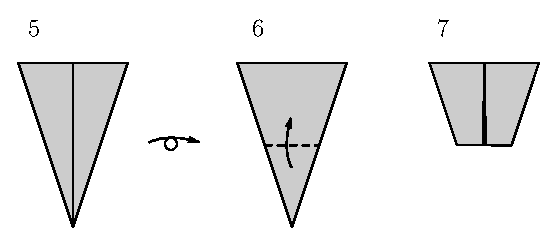
\includegraphics[scale=.98]{src/figure/chap2/fig2-8c.eps}\\
\textbf{5. ಇದನ್ನು ತಿರುಗಿಸಬೇಕು.}\\
\textbf{6. ಕೆಳಮೂಲೆಯನ್ನು ಮೇಲಿನ ಭಾಗಕ್ಕೆ ತಾಗುವಂತೆ ಮಡಚಬೇಕು.}\\
\textbf{7. ಈಗ ಒಂದು ಮಾದರಿ ತಯಾರಾಯಿತು. ಇನ್ನು ಇಂತಹ 5 ಮಾದರಿಗಳನ್ನು ತಯಾರಿಸಬೇಕು.}
\end{figure}
\begin{center}
{\bf Figure}\\
\textbf{8. ಚಿತ್ರದಲ್ಲಿ ಬಾಣದ ಗುರುತಿನ ಮಾರ್ಗದಲ್ಲಿ ಎರಡು ಮಾದರಿಗಳನ್ನು ಸೇರಿಸಬೇಕು.}\\
\textbf{9. ಎರಡು ಮಾದರಿಗಳನ್ನು ಜೋಡಿಸಿದಾಗ ಸಿಗುವ ವ್ಯವಸ್ಥೆ ಕೊನೆಯದಾಗಿ ಎಲ್ಲ ಮಾದರಿಗಳನ್ನು (Units) ಜೊಡಿಸಿದಾಗ, ನಮಗೆ "Flower for Rose" ದೊರಕುತ್ತದೆ.}
\end{center}
\begin{figure}[H]
\centering
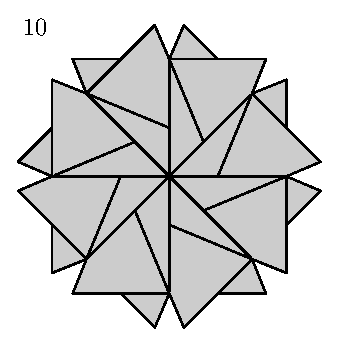
\includegraphics[scale=.98]{src/figure/chap2/fig2-8d.eps}
\end{figure}

\medskip
\noindent
{\textbf ಶೃಂಗ ಬಿಂದುಗಳುಳ್ಳ ನಕ್ಷತ್ರ [Six Point Star]}

21page processed
     
 
 
    
